\documentclass{beamer}

% don't display the beamer navbar
\usenavigationsymbolstemplate{}

\usepackage[latin1]{inputenc}
\usepackage[T1]{fontenc}
\usepackage{ae}

\mode<presentation>

%\usepackage{gb4e}
\setbeamercovered{transparent}	%fuer grau, bevor Text hinzugefuegt wird
\setbeamertemplate{blocks}[rounded][shadow=true]	%fuer abgerundete Bloecke mit Schatten

\usetheme{Warsaw}
\useoutertheme{shadow}
\usecolortheme{seagull} %overall


\title{KrdWrd - Final Presentation}
\subtitle{Dude, where is my corpus?}
\author[maria, kilian, egon]{M. Cieschinger, K. Klimek, E. Stemle}
\institute[UOS, pNLP]{Uni Osnabr\"uck, Practical NLP}
\date{July 3, 2008}

\begin{document}

\begin{frame}
	\titlepage
\end{frame}

%\begin{frame}
%	\frametitle{Outline}
%	\tableofcontents
%\end{frame}


% ... 2-3 saetze, was wir eigentlich machen
\begin{frame}
\frametitle{The Big Picture: Starting Point I}
\framesubtitle{\hfill {\tiny \cite{Evert2008,FIASCO2007}\ldots}}

	\begin{block}{Statement (Assumption)}
		The Web is an unprecedented and virtually inexhaustible source of authentic natural language data and offers the NLP community an opportunity to train statistical models on much larger amounts of data than was previously possible.
	\end{block}

\pause

	\begin{block}{Observation}
		However, after crawling content from the Web the subsequent steps, namely, language identification, tokenising, lemmatising, part-of-speech tagging, indexing, etc. suffer from 
		\begin{quote} 'large and messy' training corpora [\ldots] and interesting [\ldots] regularities may easily be lost among the countless duplicates, index and directory pages, Web spam, open or disguised advertising, and boilerplate.
		\end{quote}
	\end{block}
\end{frame}


\begin{frame}
\frametitle{The Big Picture: Starting Point II}
\framesubtitle{\hfill {\tiny \cite{Evert2008,FIASCO2007}\ldots}}
	
	\begin{block}{The Problem}
		Thorough preprocessing and cleaning of Web corpora is crucial in order to obtain reliable frequency data.
	\end{block}
	
\end{frame}


\begin{frame}
\frametitle{The Big Picture's Solution: The Mission}
\framesubtitle{\hfill {\tiny \cite{krdwrd.org}}}
	
	\begin{block}{Statement}
		The dimension of the cleaning task calls for an automated solution, the broadness of the problem for machine learning based approaches. 
	\end{block}	

\pause
	
	\begin{block}{Observation}
		Part of the KrdWrd project deals with the development of appropriate methods, but they require hand-annotated pages for training.
	\end{block}
	
\pause

	\begin{block}{The (smaller) new Problem}
		Develop a feasible way to tag content from Web pages. 
	\end{block}

\end{frame}


\begin{frame}
\frametitle{The na\"{i}ve Way of Tagging -- or CLEANEVAL-1\ldots}
\framesubtitle{\hfill {\tiny \cite{BaroniChantreeKilgarriffSharoff2008}}}

        \begin{center}
                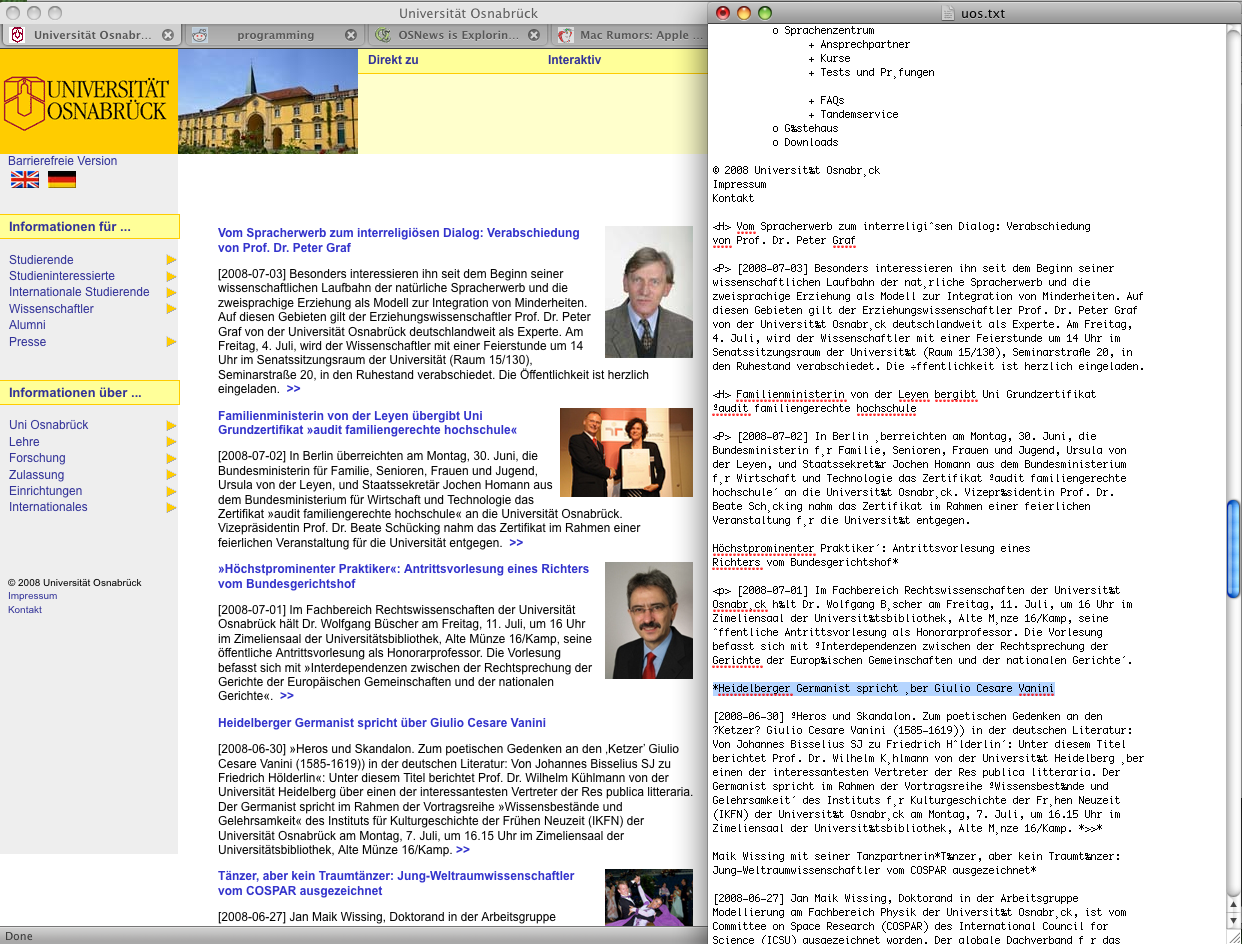
\includegraphics[width=0.8\textwidth]{20080703_pics/CleanEval.png}
        \end{center}
\end{frame}


\begin{frame}
\frametitle{Lessons Learnt -- or CLEANEVAL-2}
\framesubtitle{\hfill {\tiny \cite{BaroniChantreeKilgarriffSharoff2008}}}

	\begin{block}{Additional Requirement}
		[\ldots]participants were largely interested in using supervised machine learning techniques[\ldots and \ldots] most systems used the HTML structure of the input page as an input to their algorithms[\ldots]
	\end{block}

\pause

	\begin{block}{\ldots while being at it, namely, improving the set-up}
		preserve the \textit{structural} information of Web pages. 
	\end{block}
	
\pause
	
	\begin{block}{\ldots or even better}
		\textit{annotate} the structural information of Web pages. 
	\end{block}

\end{frame}


\begin{frame}
\frametitle{CLEANEVAL-2 and the KrdWrd Project}

	\begin{block}{}
		The KrdWrd Project includes a Firefox Add-on that aims at making this kind of tagging of Web pages possible. 
		
		\textit{For users}, we provide accurate page presentation and annotation utilities in a typical browsing environment, \textit{while preserving} the original document and all the additional information contained therein.
	\end{block}
\end{frame}


\begin{frame}
\frametitle{What We Did I}

        \begin{center}
                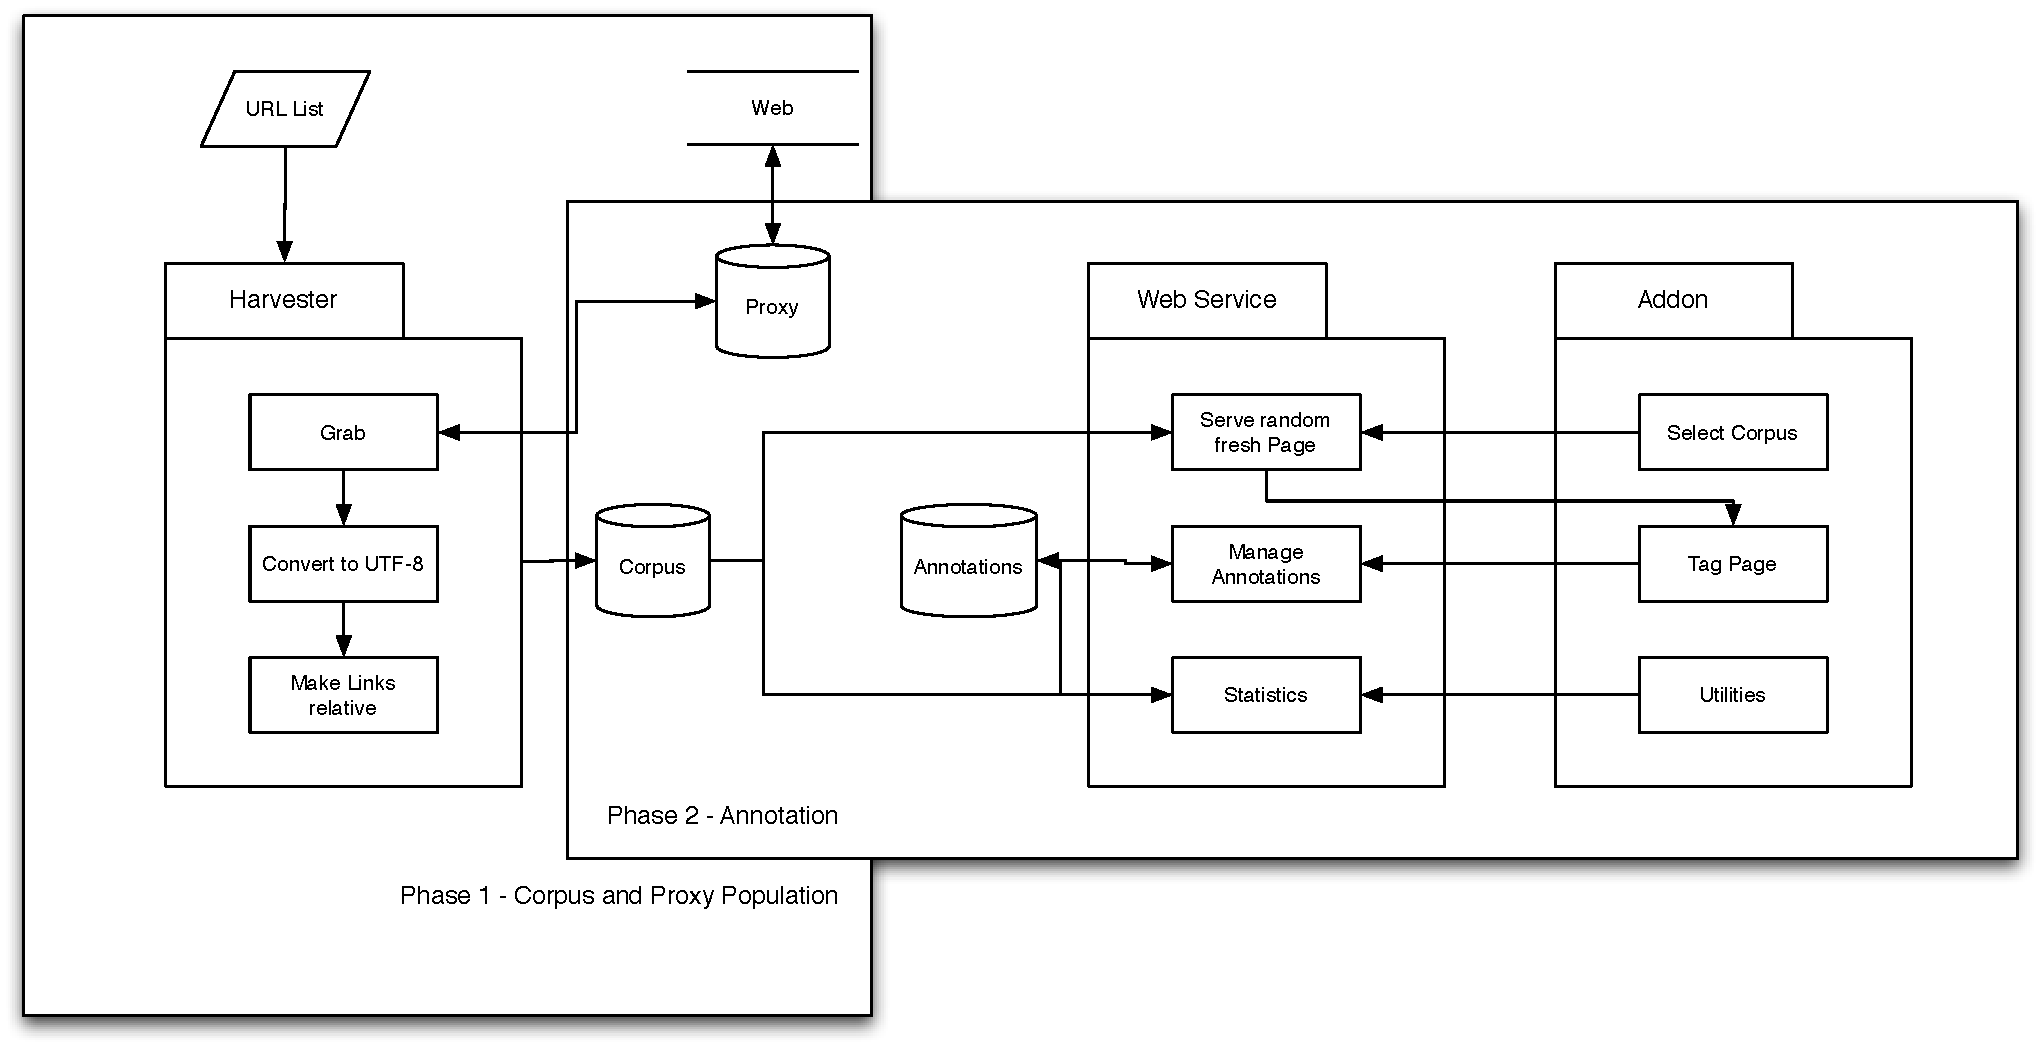
\includegraphics[width=\textwidth]{20080703_pics/corpflow.pdf}
        \end{center}

\end{frame}


\begin{frame}
\frametitle{What We Did II}
		
	\begin{block}{}
		\begin{itemize}
			\item A Firefox add-on: receive data from the server and send it back  
			\item A server: provide pages to clients and receive tagged pages (from the individual users)
			\item Refined annotation guidelines: incorporate feed-back from CleanEval-1 taggers
			\item Manual for the add-on: provide a means of getting to know the tool
			\item Interactive online tutorial: provide a means to get hands-on experience using the add-on while applying the tagging guidelines
			\item An I2CL assignment: gather Gold Standard annotations for Web pages  
		\end{itemize}
	\end{block}

\end{frame}



\begin{frame}[shrink=4]
\frametitle{How We Did It}

	\begin{block}{We Utilized}
		\begin{itemize}
			\item A shared Debian/GNU Linux Server with a shared Apache Web server
			\item A dedicated Trac, i.e.~an enhanced wiki and issue tracking system for software development projects
			\item A dedicated svn, i.e.~an open-source revision control system for all documentation and all programm code
			\item A WWWOffle proxy server to keep a (quite) pure version of the pages to be tagged
			\item A XULRunner application to harvest the pages \textit{through} the proxy -- as if they were viewed by a user
			\item JavaScript, Python, Perl, Bash-scripting for the necessary front- and back-ends
			\item A SQLite3 self-contained, embeddable, zero-configuration SQL database engine for the (less) pure version of the pages to be tagged and the users' annotations
			\item \ldots
		\end{itemize}
	\end{block}

\end{frame}

\begin{frame}{The Results}

	\begin{block}{}
		\ldots will be demonstrated \emph{LIVE}
		\url{https://krdwrd.org/screencasts/cast01.html}
	\end{block}

\end{frame}

%%%
% REFERENCES
%
%\part{References}
        %\frame{\partpage}

        %\section[references]{References}
        \begin{frame}[allowframebreaks]
                \frametitle{References}

                \setbeamertemplate{bibliography item}[text]
                \footnotesize
                \bibliographystyle{alphaurl}
                \bibliography{2008.pNLP}
                \nocite{*}
        \end{frame}
%
%%%

\end{document}
